\section{시스템 설계 및 구현}
\label{sec:system}

\subsection{아키텍처}

% JDCS: 그림 내부 내용은 영문, 캡션은 그림 아래 국문(그림 n.)+영문(Fig. n.)
\begin{figure}[t]
\centering
\begin{tikzpicture}[
  node distance=4mm and 5mm, font=\scriptsize,
  box/.style={draw, rounded corners=1pt, minimum height=6.5mm,
              minimum width=15mm, align=center, inner sep=2pt},
  arr/.style={-{Stealth[length=2mm]}}
]
  \node[box] (src) {Text source\\(melody·rhythm·lyrics)};
  \node[box, right=of src] (parser) {Parser};
  \node[box, right=of parser] (model) {Document\\model};
  \node[box, below=of model] (layout) {SVG layout\\engine (mm)};
  \node[box, left=of layout] (out) {Screen / print·PDF\\/ 300 dpi PNG};
  \node[box, left=of out] (audio) {Web Audio\\playback};
  \node[box, below=of out] (store) {localStorage /\\ \code{.jgb.json}};
  \draw[arr] (src) -- (parser);
  \draw[arr] (parser) -- (model);
  \draw[arr] (model) -- (layout);
  \draw[arr] (layout) -- (out);
  \draw[arr] (model.south west) -- (audio.north east);
  \draw[arr] (model.south) to[out=-90,in=20] (store.east);
  \draw[arr, dashed] (out.north) to[out=120,in=-60]
    node[midway, left, font=\scriptsize]{WYSIWYG editing} (src.south east);
\end{tikzpicture}
\caption{시스템 파이프라인. 텍스트 소스가 단일 원천이며, WYSIWYG 편집도
텍스트 갱신을 거쳐 동일 경로로 렌더링된다.\\
Fig.~\thefigure. System pipeline. The text source is the single source of
truth; WYSIWYG edits are also rendered through the same path via text
updates.}
\label{fig:arch}
\end{figure}

시스템은 \code{index.html}(마크업), \code{app.js}(로직, 약 4{,}100행),
\code{styles.css}(스타일)의 정적 파일 3개와, 율명 이미지·시김새 59종 SVG·
장구 구음 7종을 base64 데이터 URL로 내장한 데이터 파일 3개로 구성된다.
외부 라이브러리·서버·데이터베이스 의존이 전혀 없어 파일을 여는 것만으로
오프라인에서도 동작하며, 정적 호스팅(GitHub Pages)으로 배포된다.
이 구성은 교육 현장(설치 권한이 없는 공용 PC)과 장기 보존(플랫폼 종속성
최소화) 요구를 겨냥한 설계 결정이다.

그림~\ref{fig:arch}처럼 모든 편집은 텍스트 소스의 갱신으로 수렴하고,
파서가 이를 문서 모델로 해석하면 레이아웃 엔진이 SVG를 다시 그린다.
WYSIWYG 조작(입력 카드, 팔레트 클릭)도 내부적으로는 해당 정간의 텍스트
구간을 치환하는 것이므로, 두 입력 방식 사이에 표현 격차가 생기지 않는다.

\subsection{SVG 조판 엔진}

레이아웃은 A4 지면을 기준으로 물리 단위(mm)로 계산된다. 사용자는
한 각의 정간 수(1--64)·대강 분절·총 각 수·한 줄의 각 수·페이지당 줄 수·
정간 폭(4--30 mm)·각 간격·열 간격·머리단 등을 조정하고, 설정이 A4 인쇄
영역을 넘으면 비율을 유지한 채 자동 축소하고 축소율을 표시한다.
각은 전통 관행대로 오른쪽에서 왼쪽으로 흐르고, 대강은 프리셋
(10박=7·3, 12박=3·3·3·3, 16박=3·2·3·3·2·3, 20박=6·4·4·6) 또는 임의
분절로 굵은 선이 그어진다. 제목은 첫 페이지 오른쪽의 세로 칸(전통식)
또는 상단 가로줄로 배치할 수 있으며, 붓글씨체 등 서체·크기·자간을
지정할 수 있다. 화면 표시용 SVG와 인쇄·PNG용 SVG가 동일한 조판 결과를
공유하므로 ``보는 대로 인쇄된다''. 그림~\ref{fig:page}는 본 엔진이
조판한 A4 한 페이지의 300 dpi PNG 출력 전체이다.

\begin{figure}[t]
\centering
\fbox{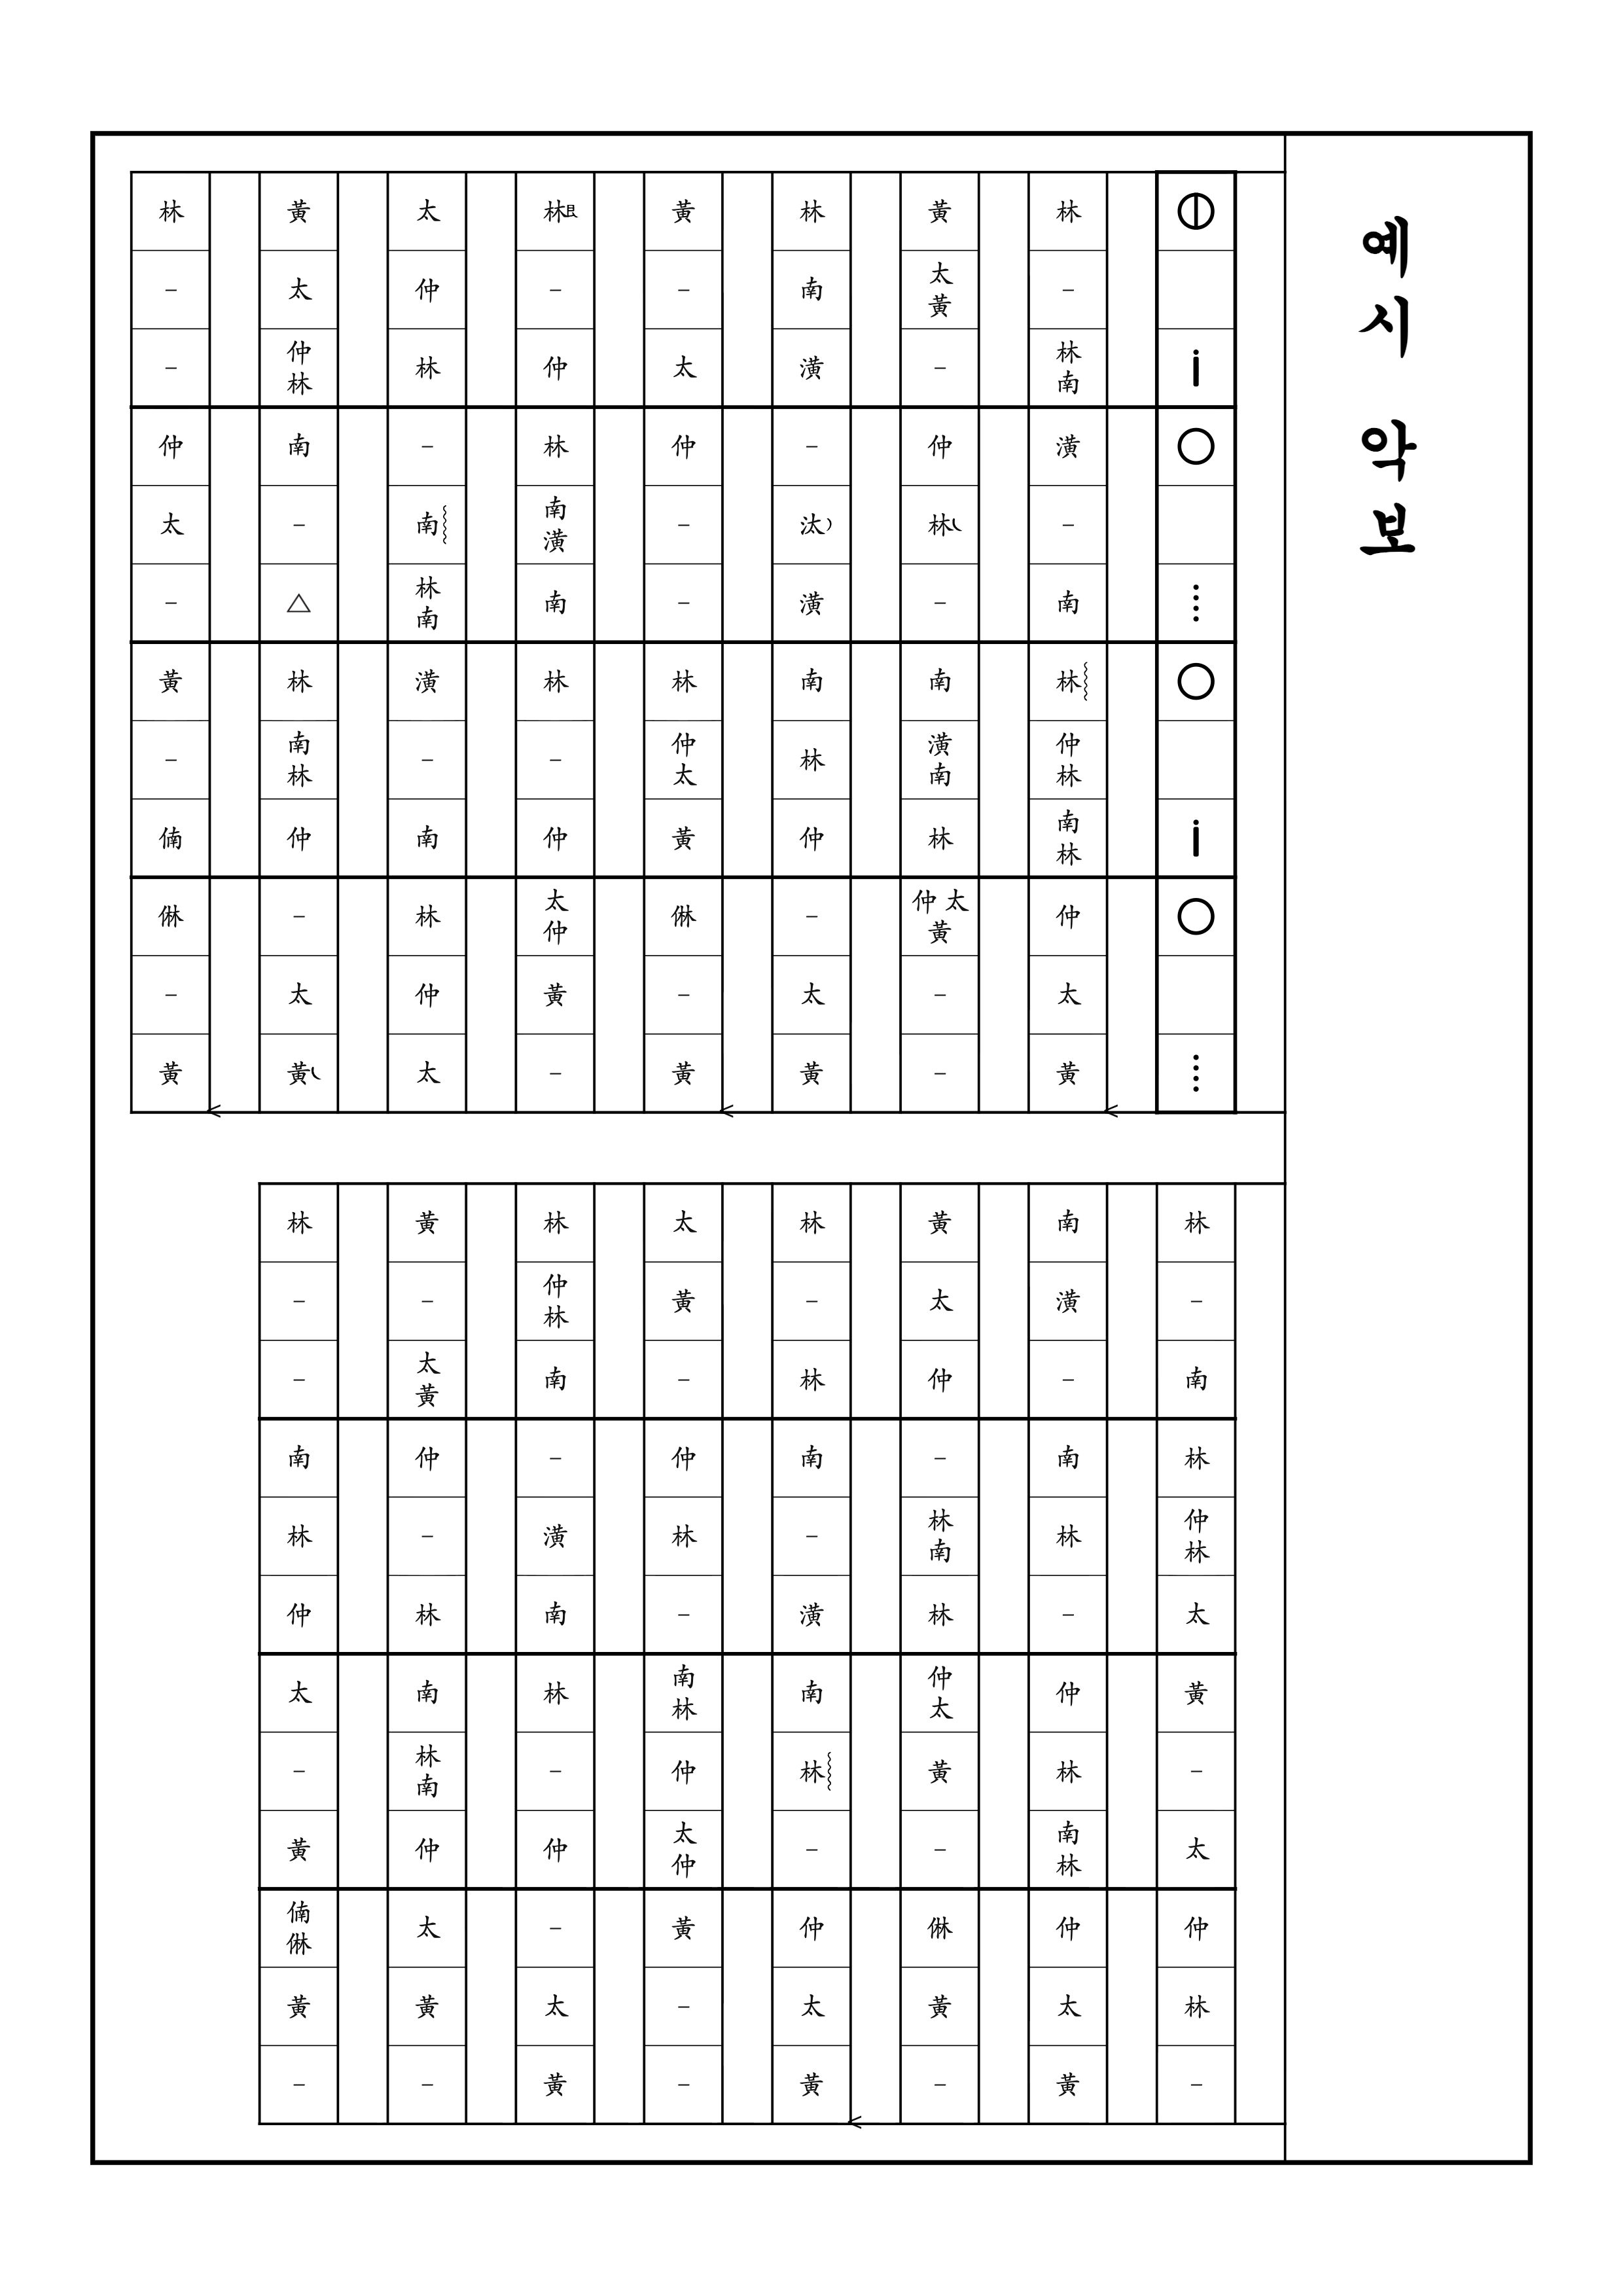
\includegraphics[width=0.86\columnwidth]{figures/fig-page.png}}

{\raggedright\scriptsize *Hangul/Hanja inside the figure is the score
content itself: jeongganbo notates pitches with Korean yulmyeong
characters.\par}
\caption{조판 결과 예 --- A4 세로, 12정간(대강 3·3·3·3), 한 줄 11칸
배치(세로 제목 칸 2 + 장단 각 1 + 선율 8각), 두 줄. 장단 각(맨 오른쪽
열)은 굵은 테두리로 선율 각과 구분되며, 각은 오른쪽에서 왼쪽으로
진행한다. 300 dpi PNG 내보내기 원본.\\
Fig.~\thefigure. Engraving example --- A4 portrait, 12 jeonggan per gak
(daegang 3·3·3·3), 11 columns per band (2 for the vertical title, 1 rhythm
gak, 8 melody gaks), two bands. The rhythm gak (rightmost column) is
distinguished by a thicker border, and gaks flow from right to left.
Original 300 dpi PNG export.}
\label{fig:page}
\end{figure}

\subsection{이중 입력과 양방향 동기화}

\textbf{직접 입력(WYSIWYG, 그림~\ref{fig:ui}).} 악보의 정간을 클릭하면
그 자리에 입력 카드가 열려 보이는 그대로 입력한다. Enter/Tab으로 다음 정간, 방향키로 인접 정간을
이동하며, 율명 팔레트(음역$\times$12율 매트릭스 또는 피아노 건반 뷰)와
시김새·장단 팔레트를 클릭해 채운다. 붙임표 시김새에는 숫자 단축키(1--0)가
배지로 표시되어, 숫자키로 고른 뒤 음을 클릭하면 즉시 부가된다.
문법을 전혀 몰라도 완전한 악보를 만들 수 있는 경로다.

\textbf{에디터(그림~\ref{fig:editor}).} 곡 전체를 텍스트로 편집한다.
각 정간 뒤에 탭을 자동 삽입해 줄이 달라도 \code{|}가 세로로 정렬되는
그리드 정렬, 해석 불가능한
토큰의 실시간 오류 표시(문법 검사), 여러 페이지 곡의 페이지 단위 표시를
제공한다. 반복 구절 복사·붙여넣기와 대량 수정에 강하다.

두 모드는 언제든 전환 가능하며, 악보에서 정간을 클릭하면 에디터의 해당
칸으로 커서가 이동하고 현재 칸이 악보에 하이라이트되는 양방향 동기화를
구현했다. 한글 입력기(IME; input method editor) 조합 중 keydown이
중복 발생하는 문제는
\code{isComposing} 가드로 처리했다.

\subsection{시김새 렌더링과 미세 조정}

시김새는 국립국악원 표기 관행을 기준으로 59종을 벡터화했다:
음표 오른쪽에 작게 붙는 붙임표 39종(미는표·흘림표·농음표 등),
한 칸을 차지하는 독립 기호 18종(전성·자출 등), 그리고 붙임·독립 양쪽으로
쓰이는 퇴성·추성 2종이다. 미세 조정 모드에서는 악보 위 시김새를 직접
클릭해 크기(40--300 \%)·좌우·상하(각 $\pm$90 \%)를 조정하고, 그 값은 3-3절의
문법으로 텍스트에 저장된다. 시김새 크기는 율명 크기 배율(0.7--2.5$\times$)과
독립적이어서 음표만 키워도 장식 기호의 균형이 유지된다.

\subsection{전통 조판 관행의 규칙화}

숙련 필사자의 지면 관행을 관찰하여 다음 규칙들을 렌더링 엔진에 명문화했다.
관찰 기준은 국립국악원 발간 악보(취타·군악 등)의 지면이다.
\TODO{기준으로 삼은 악보의 정확한 서지(간행물명·연도)를 명시하고
참고문헌에 추가할 것 --- 각주 금지 규정에 따라 본문·참고문헌으로 처리}

\begin{itemize}
  \item \textbf{이음(-) 축약}: 분박 여러 행 중 \code{-}만 홀로 있는 행은
        세로 비중을 0.68로 줄이고 남는 공간을 음표 행에 배분하여,
        지속 기호가 실제 음처럼 크게 보이지 않게 한다. \code{-} 글리프는
        가로로 1.95배 늘여 짧아 보이지 않게 하고 세로 중심을 보정한다.
  \item \textbf{2음 간격 압축}: 정간에 음이 정확히 둘이면(세로 분박이든
        가로 붙임이든) 간격을 20 \% 좁혀 성긴 인상을 막는다.
  \item \textbf{옥타브 변형 한자 우선}: 한자 모드에서는 潢(청황) 등
        변형자를 우선 쓰고, 변형자가 없는 조합에만 기본 한자에 옥타브 점을
        병기한다($\pm2$옥타브 지원). 한글 모드에서는 2글자 68 \%,
        3글자 50 \%로 자동 축소하여 칸을 넘지 않는다.
  \item \textbf{계층별 시각 구분}: 장단 각은 일반 각보다 굵은 테두리로
        둘러 선율 각과 구분하고, 반복 패턴인 장단은 곡 첫 각 옆에
        한 번만 표시한다.
\end{itemize}

\begin{figure}[t]
\centering
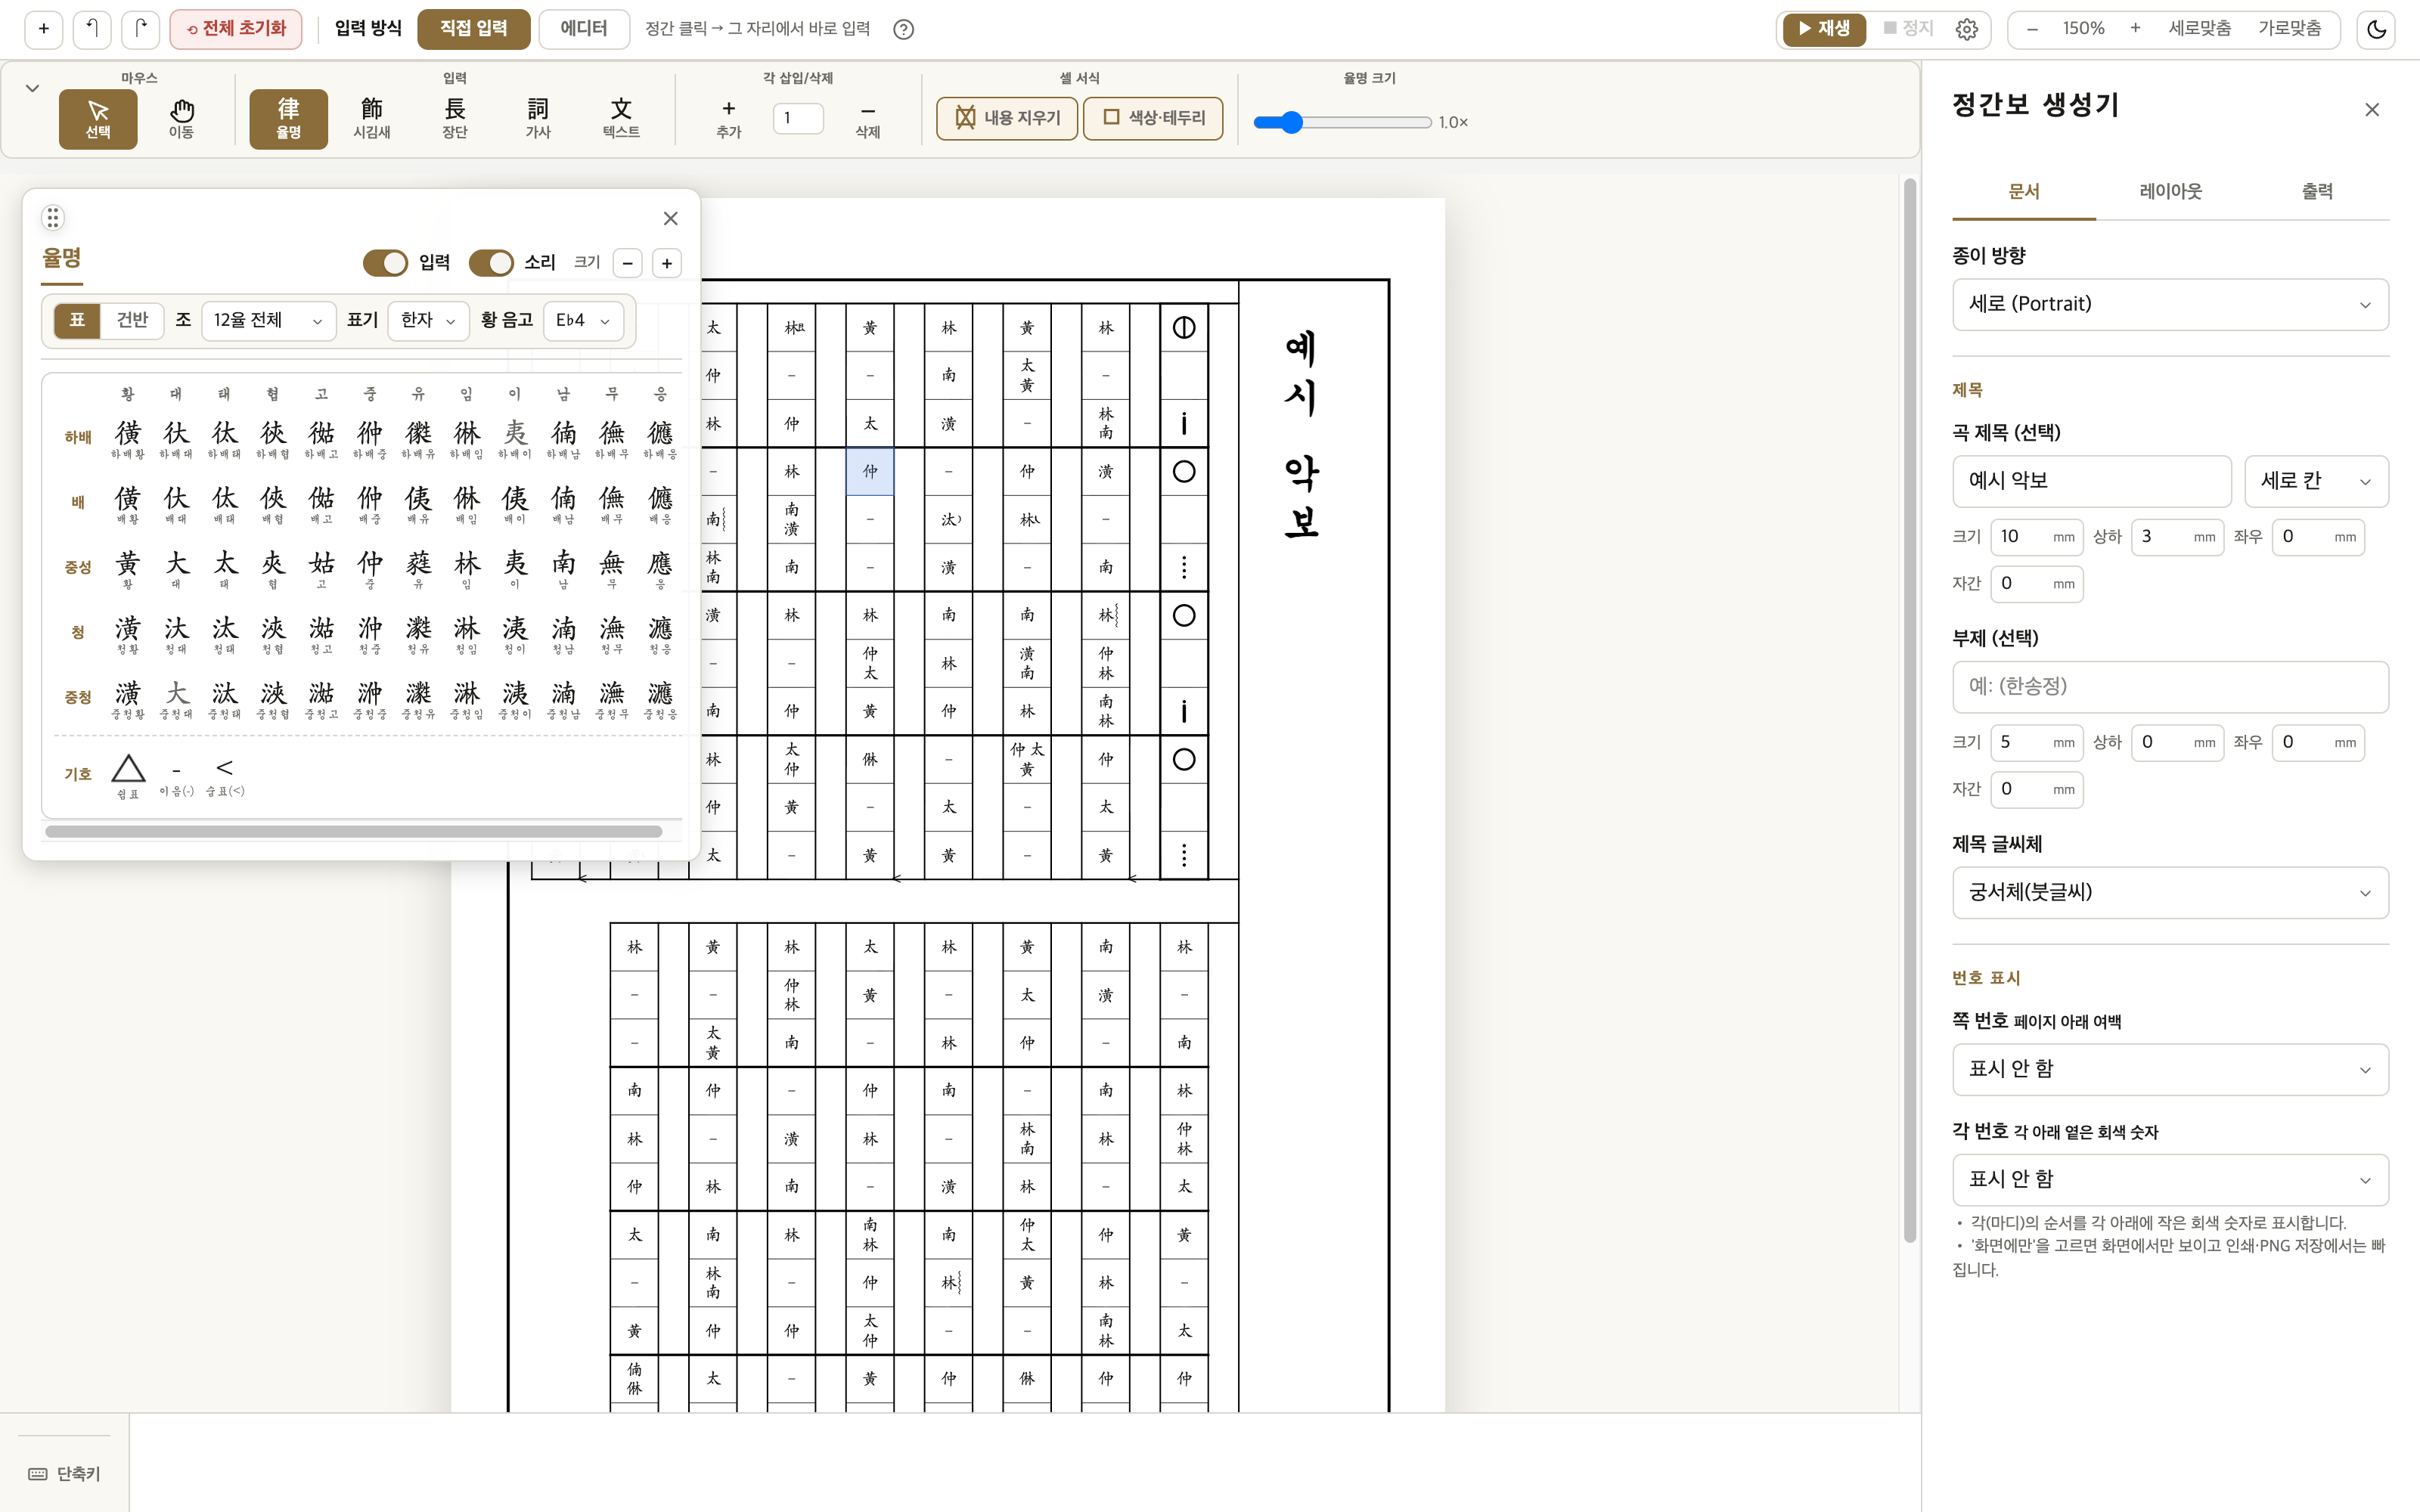
\includegraphics[width=\columnwidth]{figures/fig-ui.png}

{\raggedright\scriptsize *The UI is in Korean because the target users are
Korean traditional music practitioners; the score content itself also uses
Korean pitch-name characters.\par}
\caption{직접 입력 모드 편집 화면. 율명 도구창(음역$\times$12율 매트릭스,
한자·한글 병기)이 악보 위에 떠 있고, 클릭한 정간(파란 하이라이트)에
팔레트 선택이 바로 입력된다. 오른쪽은 문서 설정 사이드바.\\
Fig.~\thefigure. Editing screen in direct-input mode. The pitch-name
palette (register $\times$ 12 pitches, Hanja/Hangul) floats over the score;
a palette click fills the highlighted (blue) cell. The document settings
sidebar is on the right.}
\label{fig:ui}
\end{figure}

\begin{figure}[t]
\centering
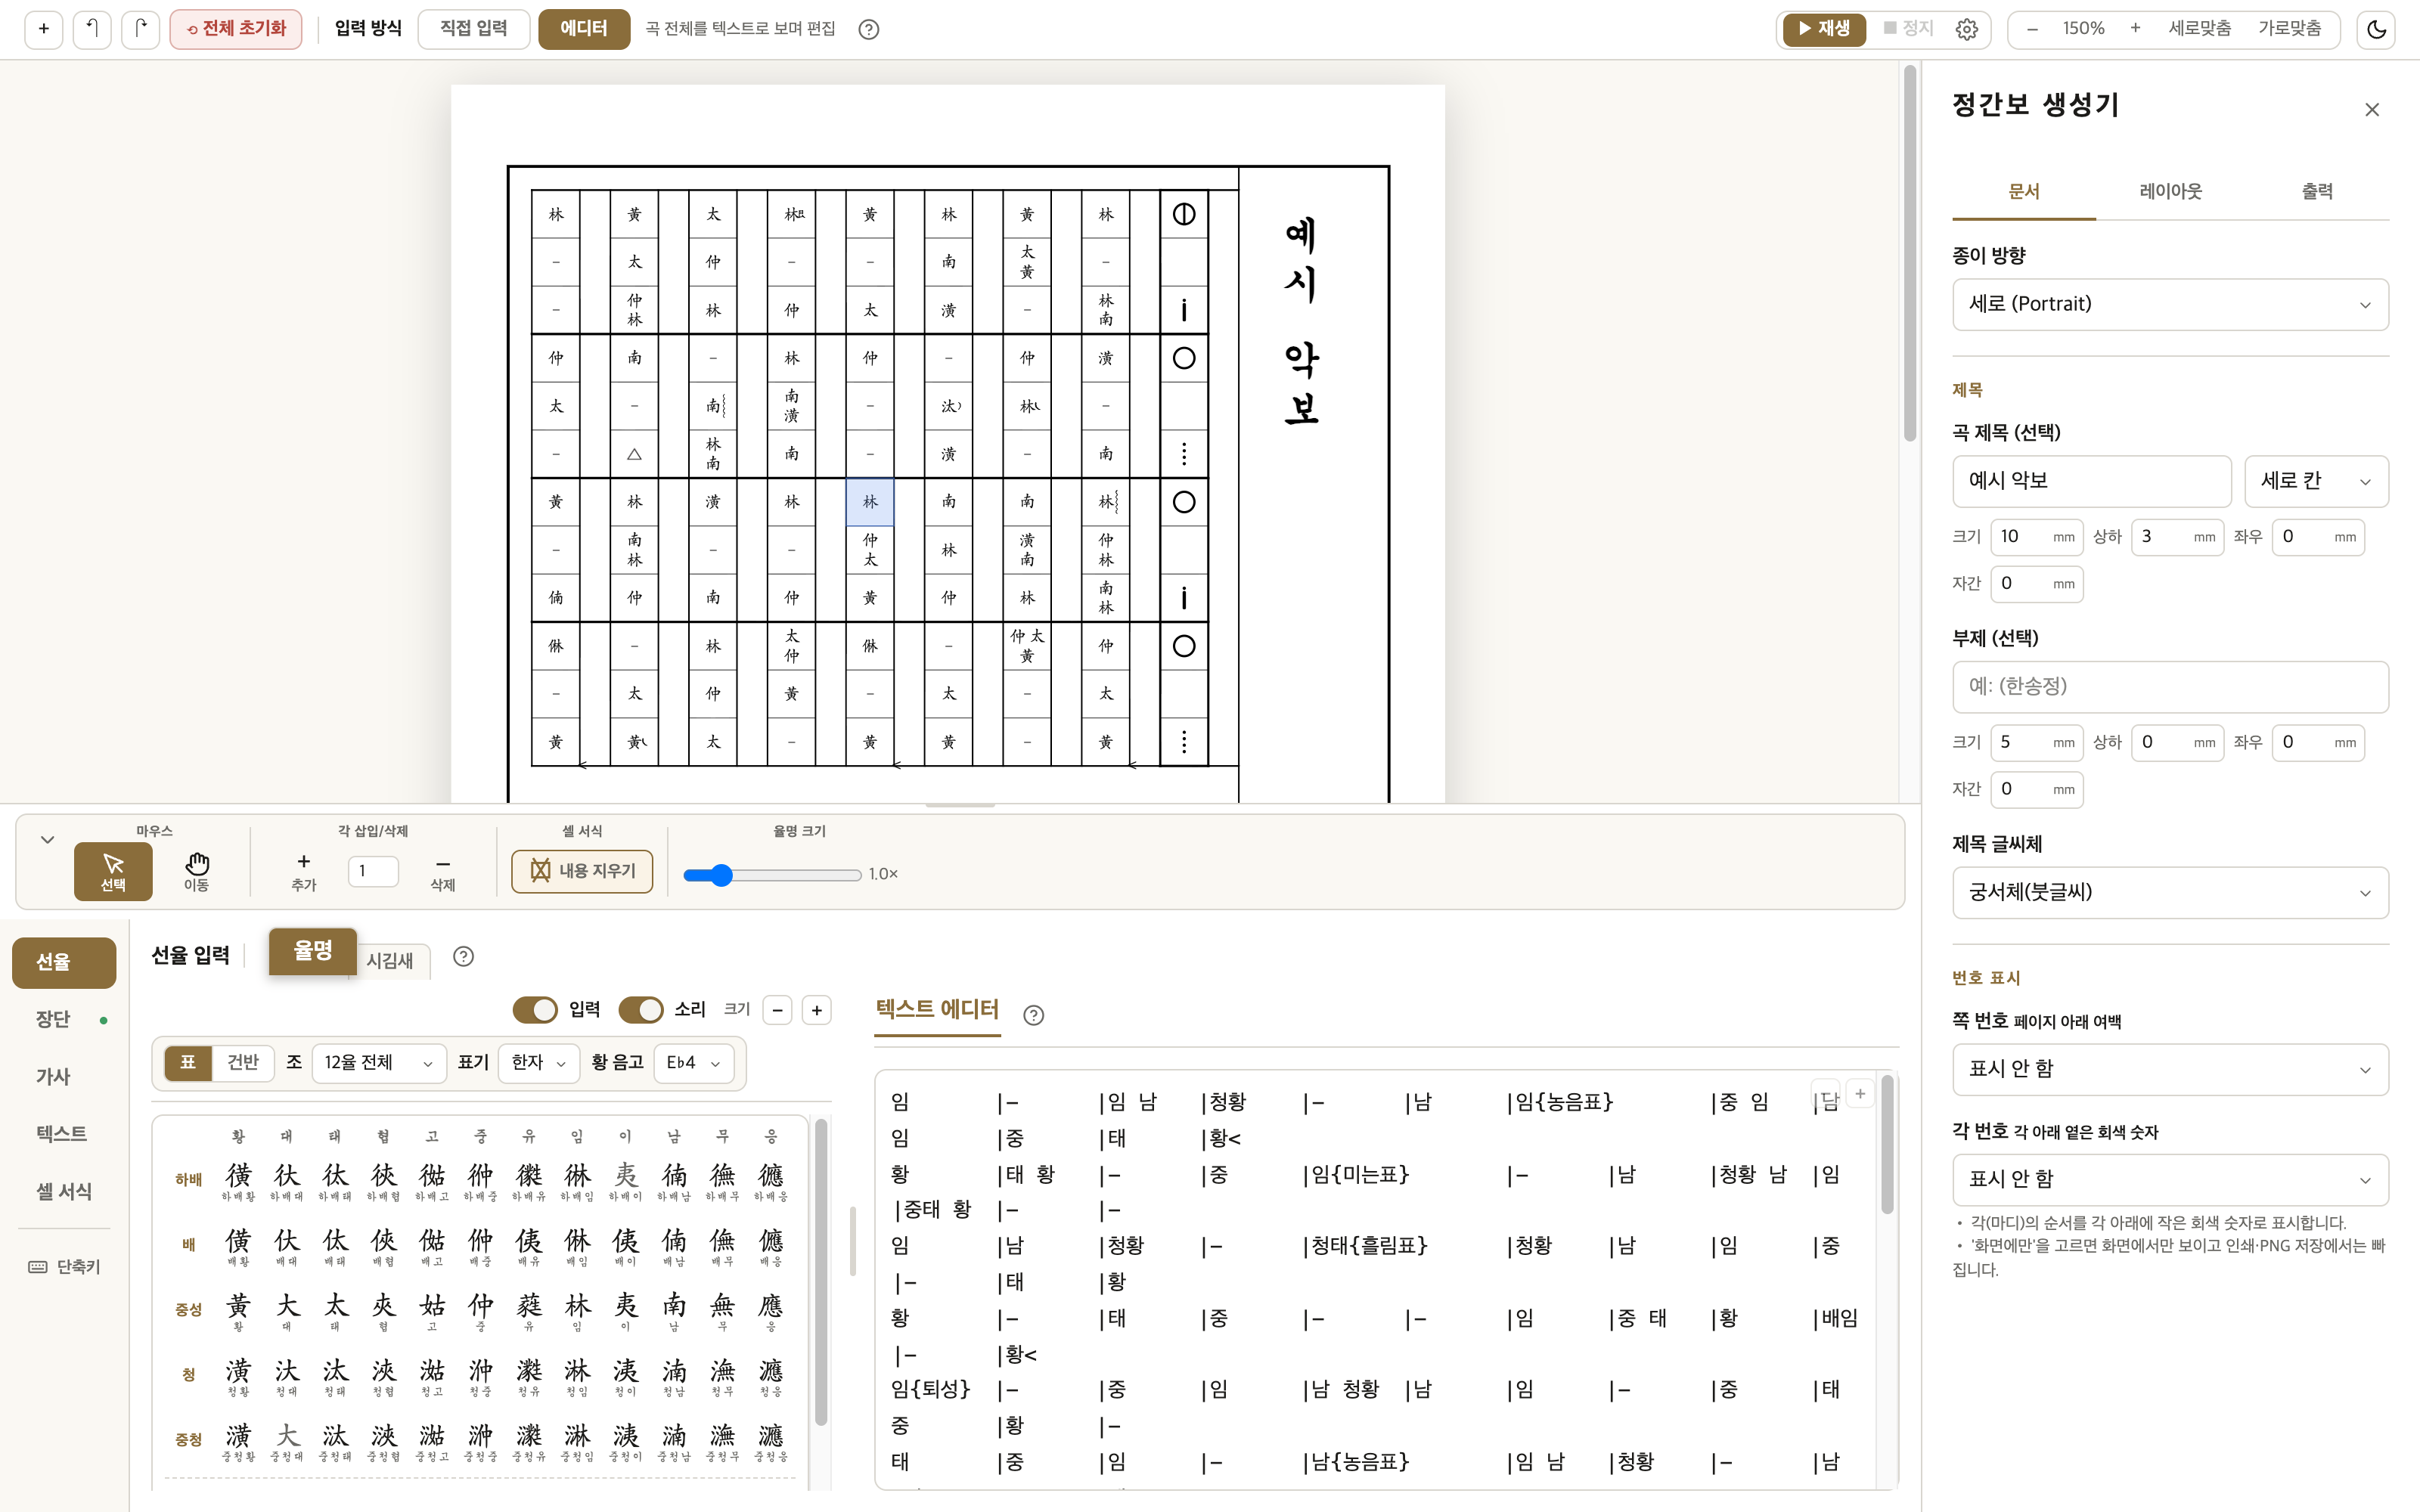
\includegraphics[width=\columnwidth]{figures/fig-editor.png}

{\raggedright\scriptsize *The UI and score content are in Korean; see the
note of Fig.~\ref{fig:ui}.\par}
\caption{에디터 모드. 아래 편집 독의 텍스트 에디터는 정간 구분자
\code{|}가 세로로 정렬되는 그리드 정렬을 제공하며, 악보에서 정간을
클릭하면 에디터의 해당 위치로 커서가 이동하고 그 정간이 악보에
하이라이트된다(양방향 동기화).\\
Fig.~\thefigure. Editor mode. The text editor in the bottom dock aligns
jeonggan separators \code{|} vertically (grid alignment); clicking a cell
in the score moves the cursor to the corresponding token and highlights
the cell (two-way synchronization).}
\label{fig:editor}
\end{figure}

\begin{figure*}[t]
\centering
\begin{minipage}[c]{0.56\textwidth}
\scriptsize
\begin{verbatim}
임|-|임 남|청황|-|남|임{농음표}|중 임|남 임|중|태|황<
황|태 황|-|중|임{미는표}|-|남|청황 남|임|중태 황|-|-
임|남|청황|-|청태{흘림표}|청황|남|임|중|-|태|황
\end{verbatim}
\end{minipage}\hfill
\begin{minipage}[c]{0.40\textwidth}
\centering
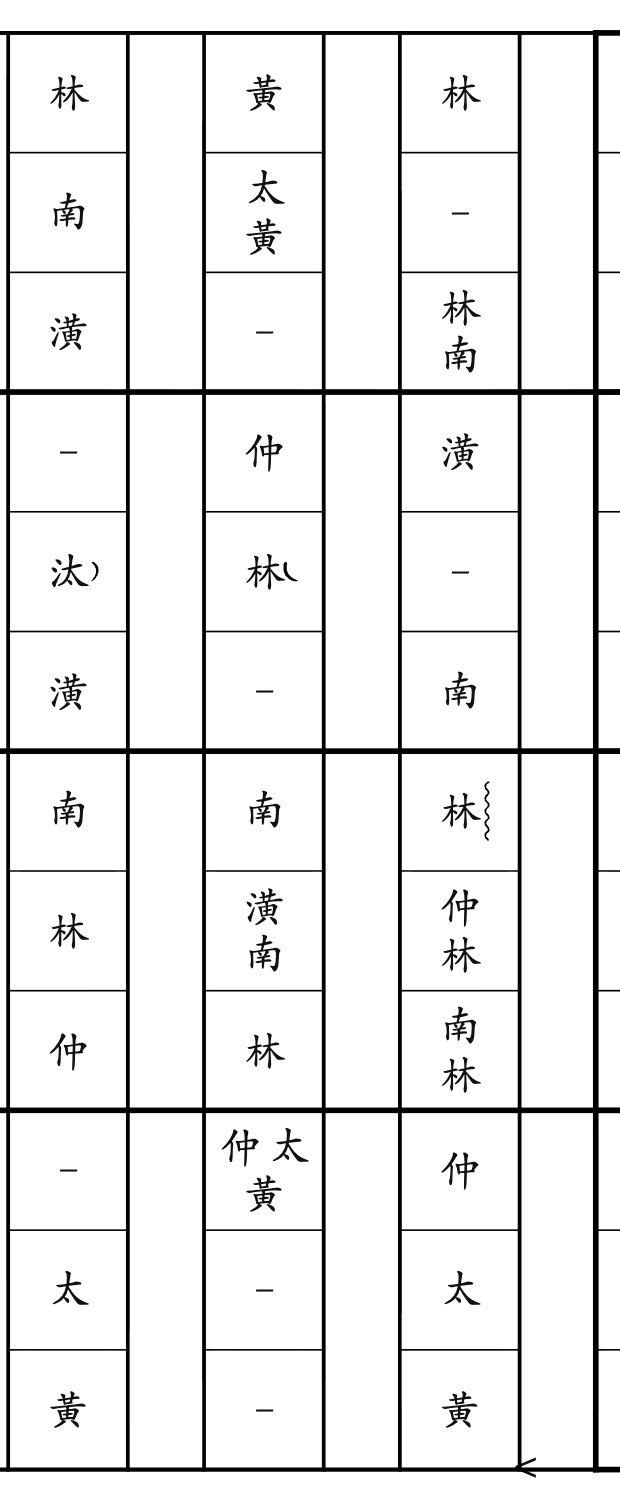
\includegraphics[height=88mm]{figures/fig-mapping.png}
\end{minipage}

{\raggedright\scriptsize *Korean characters here are the notation input
and output themselves (pitch names and ornament names).\par}
\caption{텍스트 문법(왼쪽)과 조판 결과(오른쪽)의 대응. 텍스트 첫 행이
오른쪽 그림의 맨 오른쪽 각에 해당한다(우종서). \code{|}가 정간 경계,
공백이 분박(예: 1행 셋째 정간 \code{임 남}), 연접이 붙임(2행
\code{중태 황}), \code{-}가 이음, \code{<}가 숨표로 대응되고,
시김새 \code{\{농음표\}} 등은 음표 곁의 기호로 그려진다.
굵은 가로선은 대강(3·3·3·3) 경계이다.\\
Fig.~\thefigure. Correspondence between the text grammar (left) and the
engraved result (right). The first text line maps to the rightmost gak
(right-to-left order). \code{|} marks jeonggan boundaries, spaces mark
subdivisions (e.g., \code{임 남} in line 1), juxtaposition marks horizontal
grouping (\code{중태 황} in line 2), \code{-} marks sustain, \code{<} marks
a breath, and \code{\{...\}} attaches ornaments. Thick horizontal lines are
daegang (3·3·3·3) boundaries.}
\label{fig:mapping}
\end{figure*}

\subsection{셀 서식과 편집 지원}

교육 자료 제작을 위해 정간 단위의 배경색과 변(邊) 단위 테두리
(전체/바깥쪽/안쪽 프리셋, 변 개별 선택, 3단계 굵기, 실선·점선·이중선·없음)를
지원한다. `없음'은 해당 위치의 원래 정간선까지 숨기되 악보 뼈대인 통줄과
대강선은 보호한다. 실행 취소는 문서 내용 변경만을 스냅샷(600 ms 디바운스)으로
쌓는 전역 단일 스택(Cmd/Ctrl+Z)으로 통일하여, 장단·가사 초기화나 임시 저장
불러오기까지 모두 복구된다. 다크 모드에서는 UI만 어두워지고 악보 지면은
항상 흰색을 유지해 인쇄·PNG 출력이 화면 테마와 무관하게 일정하다.

\subsection{재생}

Web Audio API로 사인파 합성 재생을 제공한다. 정간 1칸 = 1박, 분박은 등분,
빈 정간과 이음은 앞 음을 지속하며 쉼표만 무음으로 처리한다.
기준 음고는 황종 = E$\flat$4(전통 기준) 또는 C4를 선택할 수 있고
템포는 20--240 BPM(beats per minute)이다. 템포 표시를 켜면 첫 각 위에
``一分·六十井''(1분에 60정간)처럼 한자 세로 표기가 부가되는데, 이는
분당 정간 수로 빠르기를 적는 국악보 관행을 따른 것이다. 재생 중 현재
정간이 악보에 하이라이트되어 초심자의 독보(讀譜) 학습을 돕는다.

\subsection{저장과 문서 교환}

저장은 3단계다. (1) 모든 입력이 브라우저 \code{localStorage}에 즉시
자동 저장되고, (2) 이름 붙인 임시 저장 슬롯으로 여러 버전을 보관하며,
(3) 문서 전체(레이아웃 설정+선율+장단+가사+자유 텍스트+셀 서식)를
\code{.jgb.json} 파일로 내보내고 불러온다. JSON 컨테이너 안에 Ⅲ장의
텍스트 문법이 그대로 담기므로 파일은 사람이 열어 읽을 수 있고,
OMR~\cite{kim2025omr} 등 외부 파이프라인의 출력 포맷으로 쓰기에도 용이하다.
인쇄(브라우저 인쇄 대화상자를 통한 PDF 포함)와 페이지별 300 dpi PNG
다운로드를 지원한다.
